\documentclass[11pt]{article}
\usepackage[margin=1in]{geometry}
\usepackage{amsmath,amssymb,amsfonts}
\usepackage{graphicx,float}
\usepackage{fancyhdr,booktabs}
\usepackage{listings}
\usepackage{hyperref}
\usepackage{listings}
\lstset{
    language=Matlab,
    basicstyle=\ttfamily\small,
    breaklines=true,
    keepspaces=true,
    showstringspaces=false
}
\setlength{\parindent}{0pt}
% Header and Footer Setup
\pagestyle{fancy}
\fancyhf{}
\lhead{ME 300 -- Fall 2026}
\rhead{Project: Crash Attenuator}
\cfoot{\thepage}

\title{\textbf{ME 300 Project}\\[0.5ex]\Large Crash Attenuator Modeling and Analysis}
\author{Zeshui Song}
\date{Fall 2026}

\begin{document}
\maketitle
\vspace{-1em}

\section*{Overview}
The goal of this project is to model the circular aluminum hoops in a crash attenuator and determine the external force required to initiate yielding.
\begin{center}
    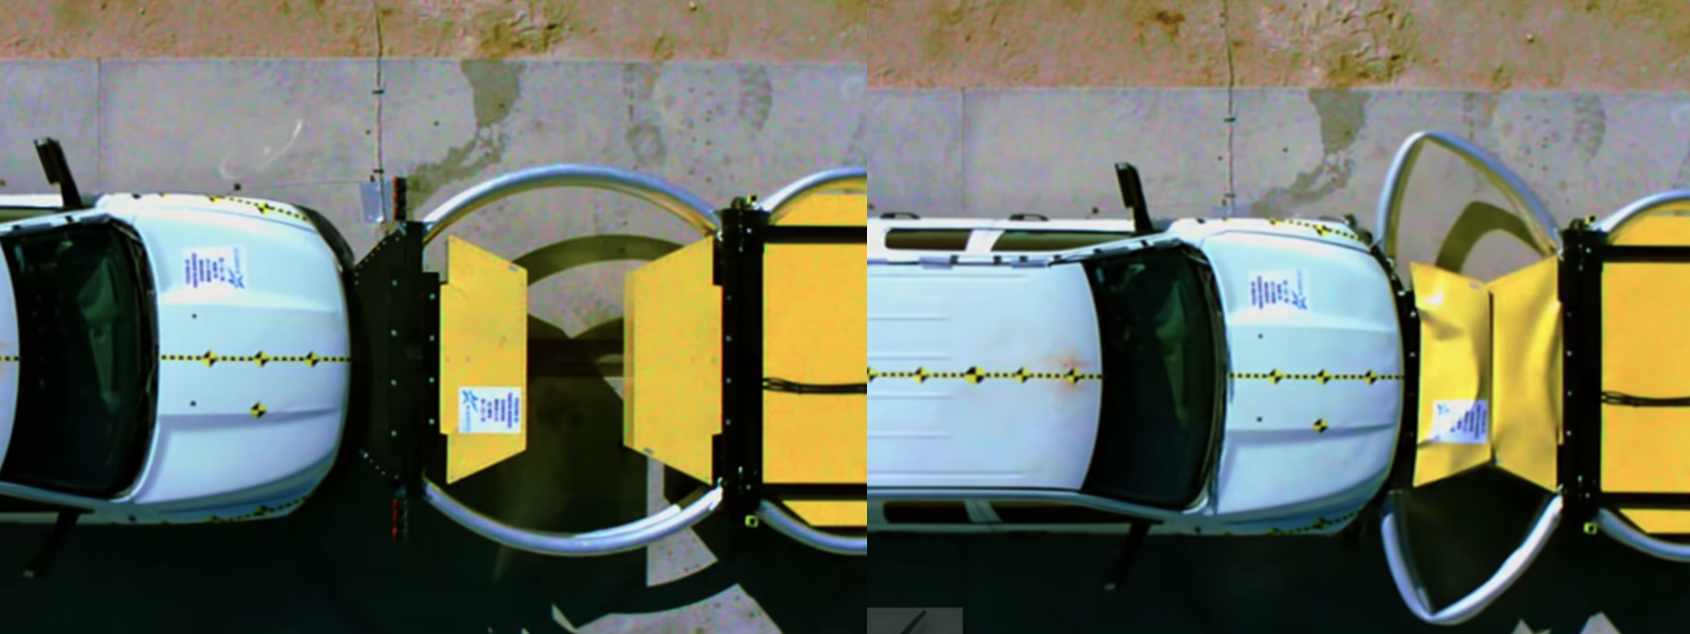
\includegraphics[width=0.5\textwidth]{Attenuator.png}
\end{center}
\begin{figure}[htbp]
    \centering
    \begin{minipage}{0.49\textwidth}
        \centering
        \includegraphics[width=\linewidth]{model full.png}
    \end{minipage}
    \hfill
    \begin{minipage}{0.49\textwidth}
        \centering
        \includegraphics[width=\linewidth]{model parts.png}
    \end{minipage}
\end{figure}
\href{https://www.traffixdevices.com/products/attenuators/scorpion2-tma\#models}{Reference: Scorpion II TMA}
\newpage
In terms of equations, we will want the relationship:
\[P \quad\rightarrow\quad M(\theta),\,N(\theta),\, V(\theta) \quad \rightarrow \quad \sigma_\theta(r,\theta)\quad\rightarrow\quad P_{yield}\]
Where:
\begin{itemize}
    \item $\theta$ is the angular position around the hoop (rad)
    \item $r$ is a radial position within the hoop cross-section (m)
    \item $P$ is the external force applied to the hoop (N)
    \item $M(\theta)$ is internal bending moment at an angular position $\theta$ (N$\cdot$m)
    \item $N(\theta)$ is internal axial force (tangent to the hoop centerline) at an angular position $\theta$ (N)
    \item $V(\theta)$ is internal shear force at an angular position $\theta$ (N)
    \item $\sigma_\theta(r,\theta)$ is the circumferential stress at a radial position $r$ and angular position $\theta$ (Pa)
    \item $P_{yield}$ is the external force required to initiate yielding (N)
\end{itemize}
For modeling purposes, assume that the second module (10002M) is rigid and fixed for smaller crashes, and the first module (10001M) is the only one that deforms. 
\begin{center}
    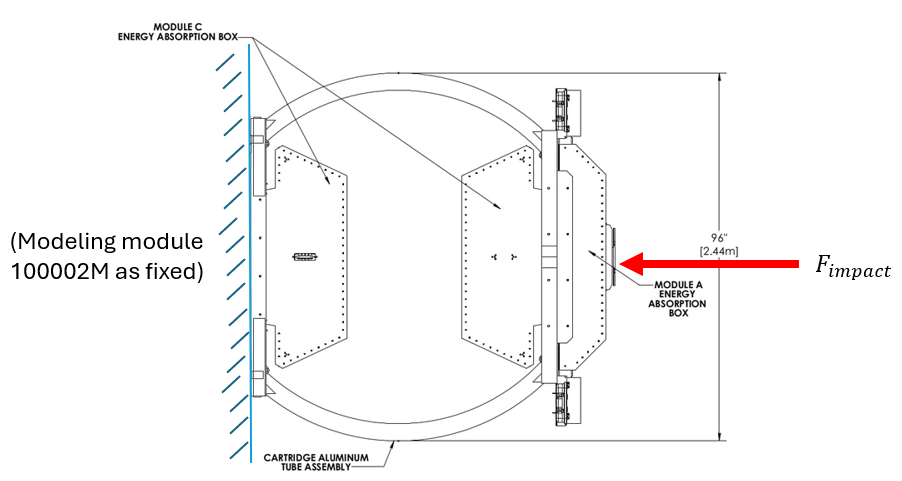
\includegraphics[width=0.8\textwidth]{Model 1.png}
\end{center}
In module 10001M, the aluminum strut is composed of 4 (approximately) circular hoops, arranged symmetrically. So we can model a single hoop that sees $1/4$ of the total impact force.
\begin{center}
    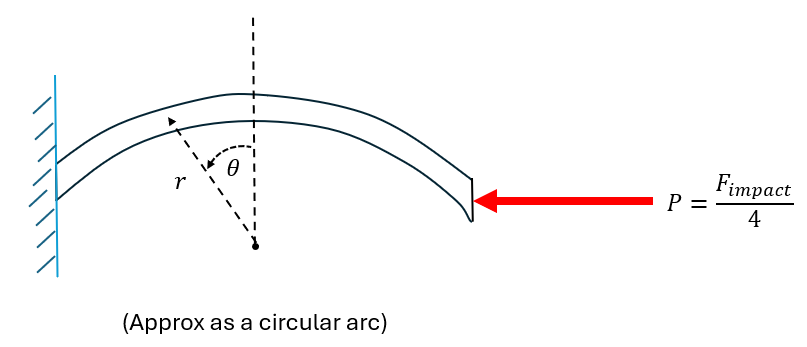
\includegraphics[width=0.8\textwidth]{Model 2.png}
\end{center}
\newpage
\section*{Deriving the Internal Load Distribution}
\subsection*{Textbook Example 10.4}
I will first derive the internal load distributions for a textbook example on page 504.
\begin{center}
    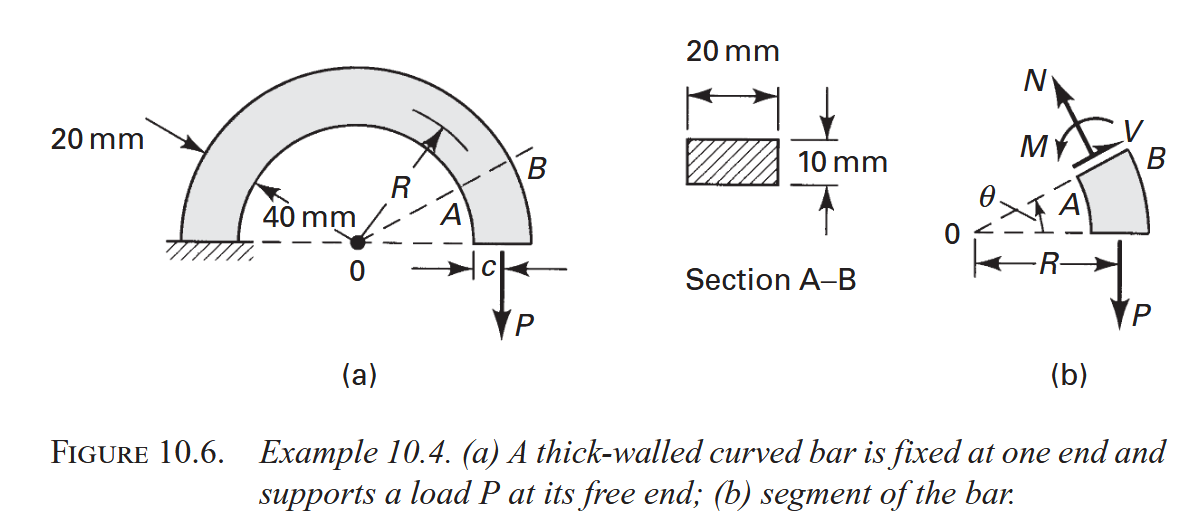
\includegraphics[width=0.8\textwidth]{Ex 10.4.png}
\end{center}
Using the free body diagram, we can derive the internal load distributions by applying the equilibrium conditions to an arbitrary section of the hoop:
\begin{center}
    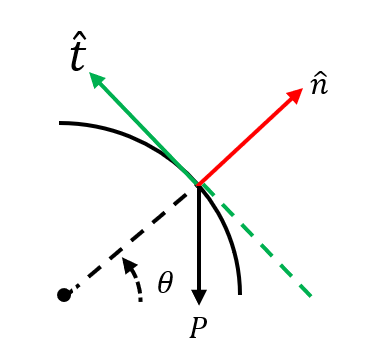
\includegraphics[width=0.25\textwidth]{coordinates .png}
\end{center}
\textbf{Tangential Equilibrium:} (in the $\hat{\theta}$ direction)
\[\sum F_t = N - P\cos\theta = 0\quad\implies\quad \boxed{N(\theta) = P\cos\theta}\]
\textbf{Normal Equilibrium:} (in the $\hat{r}$ direction)
\[\sum F_n = V-P\sin\theta = 0\quad\implies\quad \boxed{V(\theta) = P\sin\theta}\]
\textbf{Moment Equilibrium:} (about the cut face, eliminating $N$ and $V$)\\\\
From geometry, the horizontal distance from the cut face to the line of action of $P$ is:
\begin{center}
    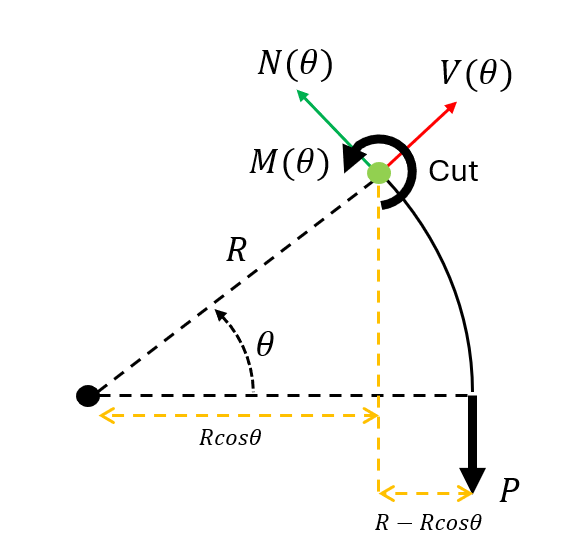
\includegraphics[width=0.3\textwidth]{geometry.png}
\end{center}
\[\sum M_{\text{cut}} = M -P(R-R\cos\theta)\quad\implies\quad \boxed{M(\theta) = PR(1-\cos\theta)}\]
\subsection*{Application to Crash Attenuator}
Following the same approach, we can derive the internal load distributions for the crash attenuator hoop. The free body diagram is shown below:
\begin{center}
    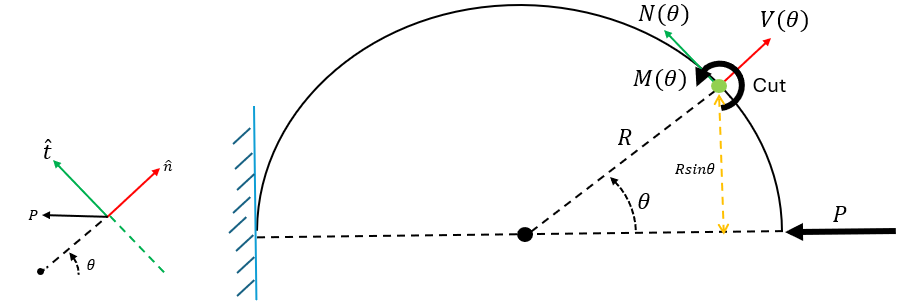
\includegraphics[width=0.8\textwidth]{geometry 2.png}
\end{center}
Isolating a section of the hoop and applying the equilibrium conditions, we have:
\[\sum F_t = N + P\sin\theta = 0\quad\implies\quad \boxed{N(\theta) = -P\sin\theta}\]
\[\sum F_n = V-P\cos\theta = 0\quad\implies\quad \boxed{V(\theta) = P\cos\theta}\]
\[\sum M_{\text{cut}} = M -P(R\sin\theta)\quad\implies\quad \boxed{M(\theta) = PR(\sin\theta)}\]
\section*{Deriving the Stress Distribution}
\subsection*{Textbook Case Study: 5.1}
Like the previous section, I will first derive the stress distribution for a textbook example on page 296.\\\\
\underline{Given:} $P = 6$ kN, $\bar{r}=50$ mm, and $h=32$ mm.\\\\
\underline{Find:} stress distribution using the curved beam formula (Winkler's formula).
\begin{center}
    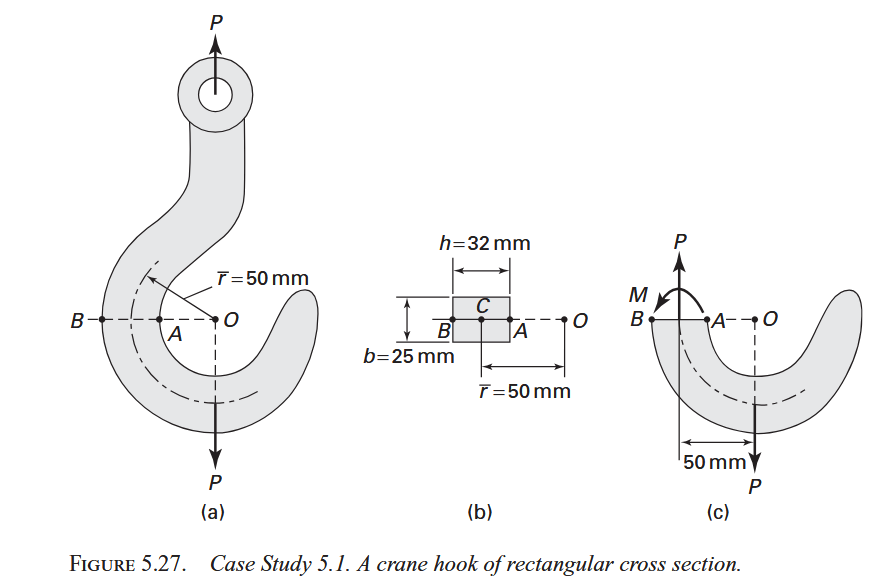
\includegraphics[width=0.6\textwidth]{Ex 5.1.png}
\end{center}
\underline{Note:} The curved beam formula accounts for the initial curvature of the beam, but assumes that plane cross-sections remain plane after bending. This assumption may not hold for our model, as the thin-walled tube can undergo cross-sectional distortion and buckling during deformation.\\\\
\textbf{Define Geometry:}
\begin{itemize}
    \item $\bar{r}$ is the radius from center of curvature ($O$) to the centroid of the cross-section ($C$)
    \item $b$ is the width of the rectangular cross-section
    \item $h$ is the height of the rectangular cross-section
\end{itemize}
\begin{itemize}
    \item Area:
    \[A=bh = 800 \text{ mm}^2\]
    \item Radii to inner and outer surfaces of the beam:
    \[r_i = \bar{r}-\frac{h}{2} = 34 \text{ mm}\]
    \[r_o = \bar{r}+\frac{h}{2} = 66 \text{ mm}\]
\end{itemize}
\textbf{Locating the Neutral Axis:}\\
The neutral axis of a curved beam doesn't pass through the geometrical centroid of the cross-section unlike for straight beams. The textbook uses eqn 5.68 to locate the neutral axis:
\[
\boxed{R_n=\frac{A}{\displaystyle\int_A \frac{dA}{r}}}
\]
Where:
\begin{itemize}
    \item $R_n$ is the radius from the center of curvature to the neutral axis
    \item $r$ is the radial position of a differential area element $dA$ within the cross-section
    \item $A$ and $dA$ are the total and differential area of the cross-section, respectively
\end{itemize}
\underline{Note:} This is valid for any cross-section, provided the assumptions of Winkler's curved-beam theory are satisfied.\\\\
For a rectangular cross-section, we can evaluate the integral:
\[dA = b \, dr\]
\[
R_n=\frac{bh}{\displaystyle\int_{r_i}^{r_o}\frac{b}{r}\,dr}=\frac{h}{\ln(r_o)-\ln(r_i)}
\]
\[
R_n=\frac{32}{\ln(66/34)}
=48.2441\ \mathrm{mm}
\]
The distance from the neutral axis to the centroid of the cross-section is:
\[\boxed{e = \bar{r} - R_n}\]
\[\implies 
e=50-48.2441=1.7559\ \mathrm{mm}
\]
\textbf{Solving for Stress Distribution}\\
We could solve for the internal loads within the beam like previously, but its too much work for an example problem. If we do have the load distribution, then we can use the curved beam formula (eqn 5.74) to solve for the stress distribution:
\[
\boxed{\sigma_\theta(r,\theta)=\frac{N(\theta)}{A}-\frac{M(\theta)(R_n-r)}{Aer}}
\]
Sign conventions:
\begin{itemize}
    \item $N>0$ is tensile axial force, $N<0$ is compressive axial force
    \item $M>0$ is counter-clockwise bending moment, producing compression at inner surface and tension at outer surface
    \item $\sigma_\theta>0$ is tensile stress, $\sigma_\theta<0$ is compressive stress
    \item $r>R_n$ is outside the neutral axis, $r<R_n$ is inside the neutral axis
\end{itemize}
\[
\underbrace{\sigma_\theta(r)}_{\text{Total normal stress}}
=
\underbrace{\frac{N}{A}}_{\text{Axial stress}}
-
\underbrace{\frac{M(R_n-r)}{Aer}}_{\text{Bending stress}}
\]
\subsection*{Application to Crash Attenuator}
While the curved beam formula only gives the normal stress distribution in the hoop, we will neglect transverse shear stress in the hoop, assuming that bending stresses dominates failure. This is supported by the fact that the hoop fails in bending (as seen in the first image of the attenuator) around the midpoint (at the top of the hoop) where the internal shear load is zero, $V(\theta=\pi/2)=0$.\\\\
\textbf{Defining Geometry:}\\
The overall diameter of the hoop is approximately $D= 2038.5$ mm. This is the average dimension $C$ in the \href{https://www.traffixdevices.com/docs/attenuators/scorpion-tma/traffix-scorpion-tma_post-impact-survey_e1.pdf}{Scorpion TMA Post-Impact Survey Measurements PDF}.\\\\
From \href{https://govtribe.com/file/government-file/7-2-dot-1-tma-mash-specifications-dot-doc}{Utah Department of Transportation (UDOT), Scorpion II TMA MASH Specifications, 2026.}, we have the following dimensions for the tube cross-section:
\begin{itemize}
    \item Tube outer diameter $d_o = 114.3$ mm
    \item Tube inner diameter $d_i = 99.06$ mm
    \item Tube wall thickness $t = 7.62$ mm
\end{itemize}
\begin{center}
    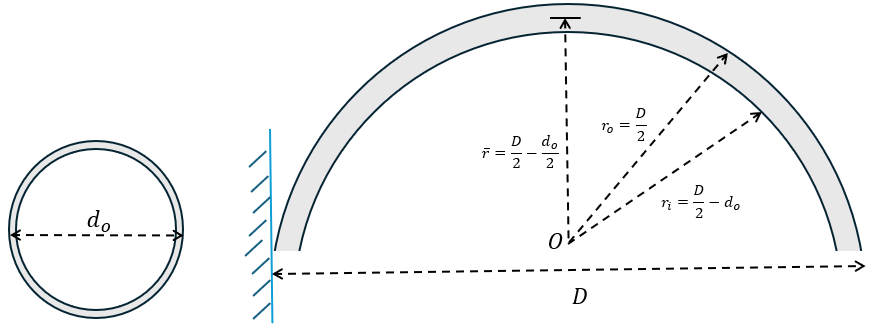
\includegraphics[width=0.8\textwidth]{crash geometry.png}
\end{center}
\begin{table}[h!]
    \centering
    \renewcommand{\arraystretch}{1.6}
    \setlength{\tabcolsep}{18pt}
    \begin{tabular}{lcc}
        \hline
        \textbf{Dimension} & \textbf{Formula} & \textbf{Value} \\
        \hline
        $\bar{r}$ & $\dfrac{D-d_o}{2}$ & $962.1 \ \mathrm{mm}$ \\
        $r_i$ & $\dfrac{D}{2}-d_o$ & $904.9 \ \mathrm{mm}$ \\
        $r_o$ & $\dfrac{D}{2}$ & $1019.3 \ \mathrm{mm}$ \\
        $A$ & $\dfrac{\pi}{4}(d_o^2-d_i^2)$ & $2553.6 \ \mathrm{mm^2}$ \\
        $d_o$ & Given & $114.3 \ \mathrm{mm}$ \\
        $d_i$ & $d_o-2t$ & $99.06 \ \mathrm{mm}$ \\
        $t$ & Given & $7.62 \ \mathrm{mm}$ \\
        \hline
    \end{tabular}
\end{table}
\textbf{Locating the Neutral Axis}
\[R_n=\frac{A}{\displaystyle\int_A \frac{dA}{r}}\]
Find the differential area element $dA = w(r)\,dr$
\begin{center}
    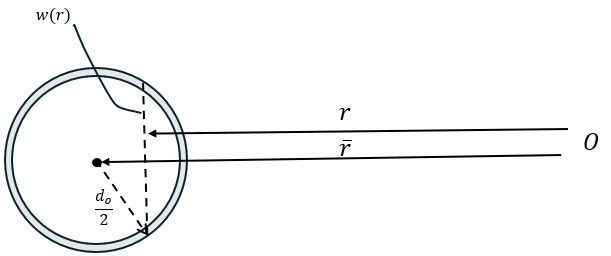
\includegraphics[width=0.5\textwidth]{differential area.png}
\end{center}
By Pythagorean theorem:
\[\left(\frac{d_o}{2}\right)^2 = (r-\bar{r})^2 + \left(\frac{w(r)}{2}\right)^2\quad \implies \quad w(r)=2\sqrt{\left(\frac{d_o}{2}\right)^2-(r-\bar r)^2}\]
Since the tube is hollow, we subtract the contribution of the inner circle from the outer circle:
\[\int_A \frac{dA}{r} = \int_{r_i}^{r_o} \frac{2\sqrt{\left(\frac{d_o}{2}\right)^2-(r-\bar{r})^2}}{r}\,dr - \int_{r_i+t}^{r_o-t} \frac{2\sqrt{\left(\frac{d_o}{2}-t\right)^2-(r-\bar{r})^2}}{r}\,dr\]
Numerical integration gives:
\begin{lstlisting}
Neutral axis radius: 960.6127 mm
Eccentricity: 1.4873 mm
\end{lstlisting}
\textbf{Solving for the Stress Distribution}
\[
\sigma_\theta(r,\theta)=\frac{N(\theta)}{A}-\frac{M(\theta)(R_n-r)}{Aer}
\]
Previously, we derived the internal load distributions:
\[N(\theta) = -P\sin(\theta),\quad M(\theta) = PR\sin(\theta)\]
Where $R = \bar{r} = 962.1$ mm is the radius from the center of curvature to the centroid of the cross-section.\\\\
Substituting into the curved beam formula:
\[
\boxed{\sigma_\theta(r,\theta)=-\frac{P\sin\theta}{2553.8}\left(1+\frac{962.1(960.613-r)}{1.4873r}\right)\quad \left[\frac{\mathrm{N}}{\mathrm{mm}^2} = \mathrm{MPa}\right]}
\]
\section*{Deriving the Yield Force}
The maximum stress according to the stress distribution occurs at $\theta = \pi/2$, evaluating the stress at this angular position for the inner and outer surfaces of the tube:
\begin{table}[h!]
    \centering
    \renewcommand{\arraystretch}{1.6}
    \setlength{\tabcolsep}{18pt}
    \begin{tabular}{lcc}
        \hline
        \textbf{Location} & \textbf{Radius} & \textbf{Stress} \\
        \hline
        Inner surface & $r_i = 904.95 \ \mathrm{mm}$ & $-0.01597P \ \mathrm{MPa}$ \\
        Outer surface & $r_o = 1019.25 \ \mathrm{mm}$ & $+0.01418P \ \mathrm{MPa}$ \\
        \hline
    \end{tabular}
\end{table}
Where $P$ is in N.\\\\
\underline{Material of Hoop:} The website states that the hoop is an aluminum tube, but does not specify the alloy. Assuming that the hoop is made of 6061-T6 aluminum, the yield strength is $\sigma_{yield} = 260$ MPa in tension.\\\\
Thus, this corresponds to a max loading of:
\[\left|\sigma_\theta(r_i,\pi/2)\right|=\sigma_{yield}\]
Substituting:
\[|-0.01597P|=260\]
Solving for the force on one hoop:
\[\boxed{P_{yield}=\frac{260}{0.01597}=16280.5\ \mathrm{N}\approx16.28\ \mathrm{kN}}\]
Since the total impact force is distributed equally among four hoops:
\[\boxed{F_{impact,yield}=4P_{yield}=65.12\ \mathrm{kN}}\]

\end{document}
